\documentclass{standalone}

\usepackage[english]{babel}
\usepackage[linesnumbered, ruled, vlined]{algorithm2e}

\usepackage{caption}

% to create listings

\usepackage{listings, lstautogobble}
\lstset{
  autogobble=true,
  frame=single,
}

\lstdefinelanguage{coq}[Objective]{Caml}{
  morekeywords={Structure, Definition, Inductive, list, return},
  sensitive=true
}

% to define font size

\usepackage{ulem}
\usepackage{moresize}
\usepackage{anyfontsize}

% to use tikz and its libraries

\usepackage{tikz-timing}
\usepackage{tikz}

\usetikzlibrary{backgrounds}
\usetikzlibrary{decorations.pathreplacing, positioning, calc, arrows, shapes, automata, petri, patterns}

% to use tikzmark, to place and refer to marks outside the current figure

\tikzset{every picture/.style={remember picture}}

% styles for transitions

\tikzset{transition/.append style={fill=black!20, thick}}
\tikzset{transition/.append style={fill=black!20, thick}}

% styles for test and inhib arcs.

\tikzstyle{test}=[pre, *-]
\tikzstyle{inhib}=[pre, o-]

% to use colors

\usepackage{xcolor}

%%%%%%%%%%%%%%%%%%%%%%%%%%%%%%%%%%%%%%%%%%%%%%%%%%
%                  BEGIN DOCUMENT                %
%%%%%%%%%%%%%%%%%%%%%%%%%%%%%%%%%%%%%%%%%%%%%%%%%%

\begin{document}

\begin{tikzpicture}


  \node (pn) {
    \begin{tikzpicture}

      \node[place] (p0) {};
      \node (pzLabel) at ($(p0)-(.7,0)$) {\ssmall $P_0$};
      
      \node[transition] (t0) at ($(p0)-(0,1)$) {};
      \node (tzLabel) at ($(t0)-(.5,0)$) {\ssmall $T_0$};
      
      \node[place] (p1) at ($(t0)-(0,1)$) {};
      \node (poLabel) at ($(p1)-(.7,0)$) {\ssmall $P_1$};

      \draw (p0) edge[post] (t0);
      \draw (t0) edge[post] (p1);
    \end{tikzpicture}
  };

  \node (vhdl) at ($(pn.east)+(3,0)$) {
    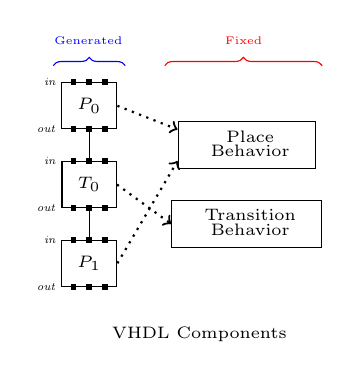
\begin{tikzpicture}

      % P0 Component + I/O
      
      \node[draw, black, inner sep=2mm] (compP0) {\ssmall $P_0$};

      \node at ($(compP0.north)-(.5,0)$) {\fontsize{4}{6}\selectfont\itshape in};
      \node[draw, black, fill=black, inner sep=.3mm] at ($(compP0.north)-(.2,0)$) {};
      \node[draw, black, fill=black, inner sep=.3mm] at (compP0.north) {};
      \node[draw, black, fill=black, inner sep=.3mm] at ($(compP0.north)+(.2,0)$) {};

      \node at ($(compP0.south)-(.55,0)$) {\fontsize{4}{6}\selectfont\itshape out};
      \node[draw, black, fill=black, inner sep=.3mm] at ($(compP0.south)-(.2,0)$) {};
      \node[draw, black, fill=black, inner sep=.3mm] at (compP0.south) {};
      \node[draw, black, fill=black, inner sep=.3mm] at ($(compP0.south)+(.2,0)$) {};

      % T0 Component + I/O
      
      \node[draw, black, inner sep=2mm] (compT0) at ($(compP0)-(0,1)$) {\ssmall $T_0$};

      \node at ($(compT0.north)-(.5,0)$) {\fontsize{4}{6}\selectfont\itshape in};
      \node[draw, black, fill=black, inner sep=.3mm] at ($(compT0.north)-(.2,0)$) {};
      \node[draw, black, fill=black, inner sep=.3mm] at (compT0.north) {};
      \node[draw, black, fill=black, inner sep=.3mm] at ($(compT0.north)+(.2,0)$) {};

      \node at ($(compT0.south)-(.55,0)$) {\fontsize{4}{6}\selectfont\itshape out};
      \node[draw, black, fill=black, inner sep=.3mm] at ($(compT0.south)-(.2,0)$) {};
      \node[draw, black, fill=black, inner sep=.3mm] at (compT0.south) {};
      \node[draw, black, fill=black, inner sep=.3mm] at ($(compT0.south)+(.2,0)$) {};

      % P1 Component + I/O
      
      \node[draw, black, inner sep=2mm] (compP1) at ($(compT0)-(0,1)$) {\ssmall $P_1$};

      \node at ($(compP1.north)-(.5,0)$) {\fontsize{4}{6}\selectfont\itshape in};
      \node[draw, black, fill=black, inner sep=.3mm] at ($(compP1.north)-(.2,0)$) {};
      \node[draw, black, fill=black, inner sep=.3mm] at (compP1.north) {};
      \node[draw, black, fill=black, inner sep=.3mm] at ($(compP1.north)+(.2,0)$) {};

      \node at ($(compP1.south)-(.55,0)$) {\fontsize{4}{6}\selectfont\itshape out};
      \node[draw, black, fill=black, inner sep=.3mm] at ($(compP1.south)-(.2,0)$) {};
      \node[draw, black, fill=black, inner sep=.3mm] at (compP1.south) {};
      \node[draw, black, fill=black, inner sep=.3mm] at ($(compP1.south)+(.2,0)$) {};

      
      \node[draw, black] (placeBehavior) at ($(compP0)!0.5!(compT0)+(2,0)$) {
        \ssmall        
        \renewcommand{\arraystretch}{.5}
        \begin{tabular}{c}
          Place\\
          Behavior
        \end{tabular}
      };

      \node[draw, black] (transitionBehavior) at ($(compT0)!0.5!(compP1)+(2,0)$) {
        \ssmall
        \renewcommand{\arraystretch}{.5}
        \begin{tabular}{c}
          Transition\\
          Behavior
        \end{tabular}
      };

      % LABEL
      \node (compLabel) at ($(compP1.south)+(1.4,-.6)$) {\ssmall VHDL Components};
      
      % EDGES
      \draw (compP0.south) -- (compT0.north);
      \draw (compT0.south) -- (compP1.north);
      \draw (compP0.east) edge[->, thick, dotted] ($(placeBehavior.west)+(0,.2)$);
      \draw (compT0.east) edge[->, thick, dotted] ($(transitionBehavior.west)$);
      \draw (compP1.east) edge[->, thick, dotted] ($(placeBehavior.west)-(0,.2)$);

      \draw[decorate, blue, decoration={brace, amplitude=3pt, raise=6pt}]
      ($(compP0.north west)-(.1,0)$) -- ($(compP0.north east)+(.1,0)$)
      node[xshift=-1.5em, yshift=1.5em] {
        \fontsize{5}{7}
        \selectfont
        \textcolor{blue}{Generated}
      };

      \draw[decorate, red, decoration={brace, amplitude=3pt, raise=6pt}]
      ($(compP0.north east)+(.6,0)$) -- ($(compP0.north east)+(2.6,0)$)
      node[xshift=-3em, yshift=1.5em] {
        \fontsize{5}{7}
        \selectfont
        \textcolor{red}{Fixed}
      };
    \end{tikzpicture}
  };

  \draw (pn.east)
  edge[double, ->, thick]
  node[yshift=1em] {
    \fontsize{5}{7}\selectfont
    \begin{tabular}{c}
      Code \\
      Generation
    \end{tabular}
    }
  (vhdl.west);
  
\end{tikzpicture}

\end{document}